\documentclass[../defence.tex]{subfiles}
\begin{document}

  \begin{frame}{Annormaler ganzzahliger Quanten Hall Effekt (QHE) in Graphen II}
    \begin{columns}[onlytextwidth, T]
      \column{\dimexpr\linewidth / 6 * 3}
        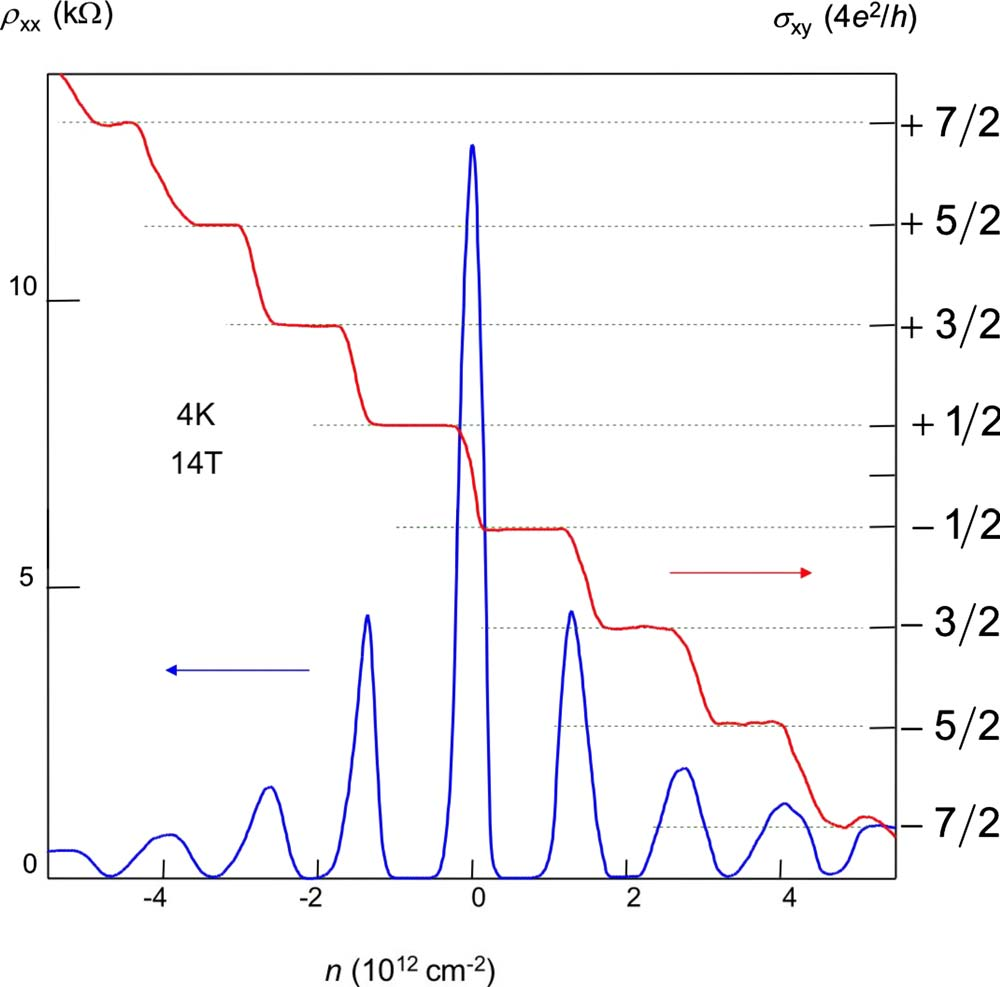
\includegraphics[width=\linewidth]{images/qhe.png}
        \cite{geim2007}
      \column{\dimexpr\linewidth / 6}
      \column{\dimexpr\linewidth / 6 * 2}
        \begin{block}{Zur Erinnerung}
          \begin{equation*}
            \rho_{xy}=\frac{\sigma_{xy}}{\sigma_{xx}^2+\sigma_{xy}^2}
          \end{equation*}
          \begin{equation*}
            \sigma_{xy}=\pm 2(2n+1)\frac{e^2}{h}
          \end{equation*}
        \end{block}
    \end{columns}
    \note{
    \begin{itemize}
      \item In blau: Longitudinalkomponente des Wiederstands
      \item In rot: Hall-Komponente der Leitfähigkeit $\rightarrow$ Kein Hall-Plateau bei $n=0$
      \item Äquidistante Stufen  der Hall-Leitfähigkeit $\sigma_{xy}$
      \item Verschiebung um $1/2$ im Vergleich zum normalen QHE
    \end{itemize}
    }
  \end{frame}

\end{document}
